\chapter{Ecosistemul Google Cloud}

\section{Alegerea platformei agentului}

Comparând Dialogflow cu alte servicii de agenți conversaționali, există mai multe caracteristici care o diferențiază și recomandă pentru utilizarea în sectorul bancar.

Dialogflow, deținut de Google, este o platformă avansată pentru dezvoltarea de aplicații de conversație, care folosește tehnologia AI pentru a interpreta intențiile și contextul utilizatorului \cite{google_dialogflow}. Aceasta oferă o gamă largă de funcționalități, inclusiv integrarea cu diverse platforme de mesagerie, asistenți virtuali și alte servicii Google, cum ar fi Google Cloud Functions.

La rândul lor, serviciile alternative, cum ar fi IBM Watson, Amazon Lex și Microsoft Luis, prezintă și ele avantaje. IBM Watson se remarcă prin puterea sa de a învăța în mod continuu și de a se adapta la diverse contexte de utilizare \cite{ibm_watson}. Amazon Lex beneficiază de integrarea nativă cu ecosistemul Amazon Web Services (AWS), oferind posibilități extinse de dezvoltare și scalare \cite{amazon_lex}. Între timp, Microsoft Luis are avantajul integrării strânse cu suita de produse Microsoft, incluzând Office 365 și Azure \cite{microsoft_luis}.

Cu toate acestea, Dialogflow se distinge prin mai multe aspecte-cheie. În primul rând, Dialogflow este foarte flexibil, permițând dezvoltatorilor să creeze experiențe de conversație personalizate pentru diferite platforme și canale de comunicare. Acesta poate fi integrat cu o multitudine de servicii, de la Google Assistant și Amazon Alexa, până la Facebook Messenger și Slack.

În al doilea rând, Dialogflow este strâns integrat cu ecosistemul Google Cloud. Acesta permite dezvoltatorilor să creeze, să testeze și să implementeze chatboti direct în cloud, profitând de avantajele cloud computing, inclusiv scalabilitatea, redundanța și accesul la cele mai recente inovații AI.

Aici intervine Google Cloud Functions \cite{google_cloud_functions}, un serviciu de calcul care permite dezvoltatorilor să execute cod ca răspuns la evenimente specifice, fără a fi nevoie să administreze o infrastructură de server. Acest serviciu poate fi utilizat în tandem cu Dialogflow pentru a crea funcții de backend pentru chatbot, cum ar fi procesarea cererilor utilizatorului, integrarea cu alte sisteme sau baze de date, sau gestionarea autentificării și a securității.

Google Cloud Functions se integrează perfect cu Google Source Repositories \cite{google_source_repositories}, un serviciu de găzduire de cod sursă care oferă un loc sigur și scalabil pentru a stoca și a gestiona codul. Acest lucru permite dezvoltatorilor să colaboreze eficient la proiecte, să gestioneze versiunile de cod și să implementeze automat codul în Cloud Functions.

În final, Google Cloud Storage oferă un serviciu de stocare de obiecte scalabil și durabil, care poate fi utilizat pentru a stoca și a servi datele utilizate de chatbot, cum ar fi înregistrări de conversații, profile de utilizator, sau alte date de context \cite{google_cloud_storage}.

\begin{figure}[h]
    \centering
    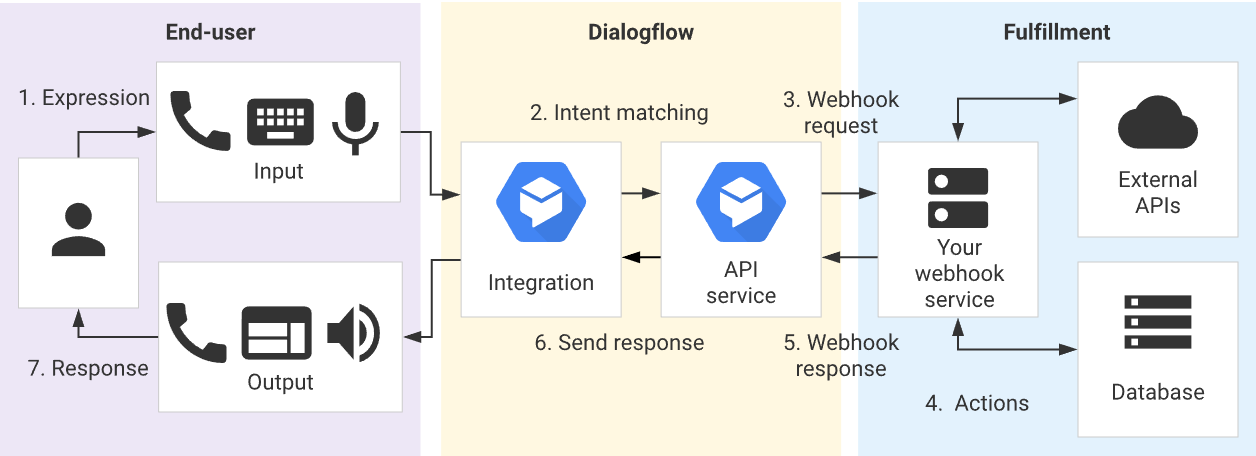
\includegraphics[scale=0.4]{fulfillment-flow}
    \caption{Flow-ul intern al Dialogflow \cite{google_dialogflow}}
\end{figure}

În ansamblu, alegerea Dialogflow, împreună cu Google Cloud Functions, Google Source Repositories și Google Cloud Storage, oferă o soluție robustă și flexibilă pentru dezvoltarea de chatboti în sectorul bancar. Prin folosirea acestor tehnologii, băncile pot crea experiențe de conversație personalizate, eficiente și securizate pentru clienții lor.

\section{Cum funcționează ecosistemul?}

Dialogflow folosește input-ul trimis de către Dialogflow API C++ Client \cite{dialogflow_client_library}, acesta fiind parsat și este trecut prin verificarea lor internă cu intențiile create în prealabil\footnote{O intenție reprezintă un anumit rezultat pe care doriți să îl obțineți de la interacțiunea utilizatorului. De exemplu, o intenție poate fi „programare întâlnire” sau „informații despre cont”.}. În funcție de cum este creat intent-ul și scopul său, pot exista parametrii scoși sub formă de entități\footnote{Entitățile sunt concepte valoroase care pot fi extrase din declarațiile utilizatorilor. De exemplu, în declarația „Doresc să programez o întâlnire pentru marți”, „marți” este o entitate de tip „dată”. Entitățile pot fi create în secțiunea „Entități” și pot fi asociate cu anumite intenții.} din textul primit (sau este un intent default, cu rol de legătură între altele cu functionalități).

\begin{figure}[h]
    \centering
    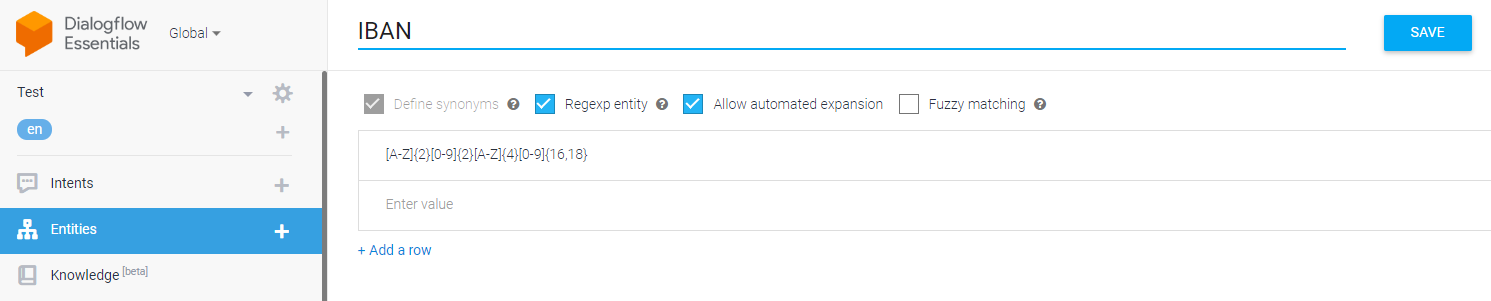
\includegraphics[scale=0.4]{entitati}
    \caption{Reprezentarea unei entități pentru IBAN folosind un regex}
\end{figure}

În cadrul platformei există niște entități predefinite \cite{system-entities} pentru a ușura munca utilizatorului atunci când vine vorba de extragere de parametrii